%; whizzy document
% latex beamer presentation.
% platex, latex-beamer でコンパイルすることを想定。 

%     Tokyo Debian Meeting resources
%     Copyright (C) 2006 Junichi Uekawa

%     This program is free software; you can redistribute it and/or modify
%     it under the terms of the GNU General Public License as published by
%     the Free Software Foundation; either version 2 of the License, or
%     (at your option) any later version.

%     This program is distributed in the hope that it will be useful,
%     but WITHOUT ANY WARRANTY; without even the implied warranty of
%     MERCHANTABILITY or FITNESS FOR A PARTICULAR PURPOSE.  See the
%     GNU General Public License for more details.

%     You should have received a copy of the GNU General Public License
%     along with this program; if not, write to the Free Software
%     Foundation, Inc., 51 Franklin St, Fifth Floor, Boston, MA  02110-1301 USA

% 実行順番
% sudo  ~/bin/usb-macbook-ir.c &
% real presentation (shell-command (concat "DISPLAY=:0.1 xpdf -fullscreen " (replace-regexp-in-string "tex$" "pdf"(buffer-file-name)) "&"))
% DISPLAY=:0.1 xpdf -fullscreen 

\documentclass[cjk,dvipdfmx]{beamer}
\usetheme{Warsaw}
%  preview (shell-command (concat "xpdf " (replace-regexp-in-string "tex$" "pdf"(buffer-file-name)) "&"))
%  presentation (shell-command (concat "xpdf -fullscreen " (replace-regexp-in-string "tex$" "pdf"(buffer-file-name)) "&"))


%http://www.naney.org/diki/dk/hyperref.html
%日本語EUC系環境の時
\AtBeginDvi{\special{pdf:tounicode EUC-UCS2}}
%シフトJIS系環境の時
%\AtBeginDvi{\special{pdf:tounicode 90ms-RKSJ-UCS2}}

\title{東京エリア Debian 勉強会}
\subtitle{資料}
\author{上川 純一 dancer@debian.org\\IRC nick: dancerj}
\date{2006年8月19日}
\logo{
\includegraphics[width=8cm]{image200607/openlogo-light.eps}}

% 三択問題用
\newcounter{santakucounter}
\newcommand{\santaku}[5]{%
\addtocounter{santakucounter}{1}
\frame{\frametitle{問題\arabic{santakucounter}. #1}
%問題\arabic{santakucounter}. #1
\begin{minipage}[t]{0.7\hsize}
 \begin{itemize}
 \item  A #2\\
 \item  B #3\\
 \item  C #4\\
 \end{itemize}
\end{minipage}
}
\frame{\frametitle{問題\arabic{santakucounter}. #1}
%問題\arabic{santakucounter}. #1
\begin{minipage}[t]{0.7\hsize}
\begin{itemize}
\item  A #2\\
\item  B #3\\
\item  C #4\\
\end{itemize}
\end{minipage}
\begin{minipage}[t]{0.2\hsize}
答えは:


\vspace{1cm}

{\huge \hspace{1cm}#5}
\end{minipage}}
}


\begin{document}
\frame{\titlepage{}}

\section{Intro}
\begin{frame}
 \frametitle{本日のagenda}
\begin{itemize}
 \item 注意事項
       \begin{itemize}
	\item 飲食禁止
	\item 政治/宗教/営利活動禁止
       \end{itemize}
 \item Social Contract 唱和
 \item 事前課題紹介
 \item quiz
 \item Debian Conference 進捗報告
 \item Lightening Talks
\end{itemize}
\end{frame}

\subsection{祝13執念}
\begin{frame}
 \frametitle{祝13執念}
 \begin{itemize}
  \item 8/16: Debian 13年目の誕生日
 \end{itemize}
\end{frame}

\subsection{Social Contract唱和}
\begin{frame}
\frametitle{1. Debian will remain 100\% free} 

       We provide the guidelines that we use to determine if a work is
       "free" in the document entitled "The Debian Free Software
       Guidelines". We promise that the Debian system and all its
       components will be free according to these guidelines. We will
       support people who create or use both free and non-free works on
       Debian. We will never make the system require the use of a
       non-free component.
\end{frame}
\begin{frame}
\frametitle{2. We will give back to the free software community} 
 
    
       When we write new components of the Debian system, we will license
       them in a manner consistent with the Debian Free Software
       Guidelines. We will make the best system we can, so that free
       works will be widely distributed and used. We will communicate
       things such as bug fixes, improvements and user requests to the
       "upstream" authors of works included in our system.
\end{frame}
\begin{frame}
\frametitle{3. We will not hide problems} 
 

       We will keep our entire bug report database open for public view
       at all times. Reports that people file online will promptly become
       visible to others.
\end{frame}
\begin{frame}
\frametitle{4. Our priorities are our users and free software} 
       We will be guided by the needs of our users and the free software
       community. We will place their interests first in our priorities.
       We will support the needs of our users for operation in many
       different kinds of computing environments. We will not object to
       non-free works that are intended to be used on Debian systems, or
       attempt to charge a fee to people who create or use such works. We
       will allow others to create distributions containing both the
       Debian system and other works, without any fee from us. In
       furtherance of these goals, we will provide an integrated system
       of high-quality materials with no legal restrictions that would
       prevent such uses of the system.
\end{frame}
\begin{frame}
\frametitle{5. Works that do not meet our free software standards} 
    
       We acknowledge that some of our users require the use of works
       that do not conform to the Debian Free Software Guidelines. We
       have created "contrib" and "non-free" areas in our archive for
       these works. The packages in these areas are not part of the
       Debian system, although they have been configured for use with
       Debian. We encourage CD manufacturers to read the licenses of the
       packages in these areas and determine if they can distribute the
       packages on their CDs. Thus, although non-free works are not a
       part of Debian, we support their use and provide infrastructure
       for non-free packages (such as our bug tracking system and mailing
       lists).
\end{frame}


\section{事前課題の声}

\begin{frame}
 \frametitle{ユーザの声}
自分は元々redhat9からLinuxを使い始めた人間なのですが
apt・dpkgやupdate-alternatives・kernel-package等のシステム管理のパッケージが気に入っています。
独自の使い方やルール等の感覚をつかむまでよくわかりませんでしたが
これらのパッケージの存在のお陰でシステムの基盤をお好みに構築するのは
他ディストリビューションと比べても結構スムーズに出来る気がします。
{\em システムの依存関係もめちゃくちゃになりにくいのも助かっています。}
\end{frame}

\begin{frame}
 \frametitle{ユーザの声}
私が、最近感銘を受けたパッケージは、現在Debianのオフィシャルパッケージではないが、
howm(一人お手軽Wikiもどき)だ。ソースファイルを見てみたら、
GPLだと書かれていてユーザーも多いみたいなので、
{\em 将来的にはDebianのオフィシャルパッケージになるのではないかと思う。}
大学に入るまでは、PDAであるVisorEdgeを使って、予定やちょっとしたメモを取ってきたが、
Linuxを本格的に使うようになってから、コマンドが多く適当にディレクトリーを使って、
雑文を保存していた。しかし、最近検索機能などもつけたいし、
予定やtodoとしての機能も使いたいので何かEmacs上で良いソフトがないか調べていたら、
howmを知った。howmは、リンク機能、そして検索機能などもあり、
メモを書くにはかなり便利なソフトだと思われる。
\end{frame}

\begin{frame}
 \frametitle{ユーザの声:添削後}
私が、最近感銘を受けたパッケージは、現在Debianのオフィシャルパッケージではないが、
howm(一人お手軽Wikiもどき)だ。ソースファイルを見てみたら、
GPLだと書かれていてユーザーも多いみたいなので、
{\em 将来的にはわたしがDebianのオフィシャルパッケージにする予定。}
大学に入るまでは、PDAであるVisorEdgeを使って、予定やちょっとしたメモを取ってきたが、
Linuxを本格的に使うようになってから、コマンドが多く適当にディレクトリーを使って、
雑文を保存していた。しかし、最近検索機能などもつけたいし、
予定やtodoとしての機能も使いたいので何かEmacs上で良いソフトがないか調べていたら、
howmを知った。howmは、リンク機能、そして検索機能などもあり、
メモを書くにはかなり便利なソフトだと思われる。
\end{frame}

\begin{frame}
 \frametitle{ユーザの声}
    「Debian 誕生日」って具体的には何時だろう?
・・・という事で、Google 様に聞いてみてみると、
「Debian 5 回目の誕生日!」という1998年08月13日の
Debian ニュースの記事が見つかった。  と言う事は
1993年08月16日が誕生日って事ですね。

    13 歳というと、人間で言えば小学校卒業して中学
生になった頃でしょうか?  人間ならばこの頃には、相
手がアホでも相手に合わせて会話が出来るようになるの
で、Debian も私のようなアホにも愛想良く簡単に使え
るようになって頂ければ嬉しいなぁ〜、と思います。

    なにはともあれ、13 年目、めでたい事であります。
\end{frame}

\begin{frame}
 \frametitle{ユーザの声}

なんだかしらないが時間ばっかり過ぎている自分と比べて徐々に
成長しているような気がする「Debian」はすごいなぁと思う。

最初期から活動してきた人とかはどんどん減って
新しい人がどんどん入っているのかなぁ(日本除く)と思う。

13周年というと、徐々に枯れたプロジェクトになって行くのだろうか?

13歳と言うともう中学生、つまり「チュウボウ」なので、反抗期みたいな
尖ったプロジェクトになって行くのだろうか?

今年(?)はetchをリリースするようだけど今後の安定的なリリースのために
大きな一歩になる年になるのだろうか。

今年も楽しみなプロジェクトです。
{\em 今年こそもう少しなんかできるといいなぁ。}
\end{frame}

\begin{frame}
 \frametitle{ユーザの声}
13周年ですか、13年前はまだDOSとWindowsしか知らなかったです。
Debianは使いはじめて2年強、Linux自体もまだ5年そこそこの新参者なので恐縮ですが、
今後ますます発展してほしいです。{\em まずは自分の周りの人間を引き込むところから始めます。}
\end{frame}

\begin{frame}
 \frametitle{ユーザの声}
あれはたしか小学校高学年、あるいは中学校に入学した直後だったと思
う。
ちょうど算数・数学でxを用いた方程式を学習する時期であった。
導入として以下のような問題の解き方を考えさせられた。
同じような問題を解かされた方も少なくないと思う。

龍三郎さんは現在47歳です。
香織さんは21歳です。
龍三郎さんの年齢が香織さんの年齢のちょうど倍になるのは何年後でしょ
う。

答えは以下の方程式を解くことで求められる:

$47+x=2(21+x)$, 
$x=5$

さてDebian は13歳の誕生日だそうだが、Debianの年齢とみなさんの年齢を用いてこの
方程式を組み立て、解いてみていただきたい。
今、日本のDebian 開発者、OSS開発者に特に求められているのは$x<0$の人材で
はないだろうか。
$x<0$ の方々には堂々と胸を張って大いにあばれていただきたい。
\end{frame}

\begin{frame}
 \frametitle{ユーザの声}
かくいう私は$x=3$です。
失礼しました。
\end{frame}

\begin{frame}
 \frametitle{ユーザの声}
数年前までは Debian? Linux? ハァ? と言う感じでしたが、今ではどっぷり使って Debian を
開発する側に回ってしまいました。今ではもっと先に Debian と戯れていたらなぁと思っています。
{\em 13 終年} にならないよう、今後もがんばっていけたらなぁと思います。
\end{frame}

\begin{frame}
 \frametitle{ユーザの声}
忘れもしないCマガジン1995年10月号特別付録CD-ROMに収録されていた
Linux/TOWNSから始まったLinux生活。本誌に掲載されていたLinux解説記事の
著者が鵜飼さんだったことはDebianに繋がる見えない道標だったのでしょうか。

13年の歴史の中で様々の障害に取り掛かり乗り越えてきたのだと思います。
ソフトウェア特許は難しいながら長年の課題としてあり続けてきたものですが、
私にとって予想外だったのはFDLとの衝突でしょうか。GPLv3も今年中にはっきり
とした形を見せてくる予定だったと思います。

これからもオープンソースライセンスに関してDebianの主導的振舞に
期待しています。
\end{frame}

\section{DWNQuiz}
%% debianmeetingresume200608.texから以下コピー

\subsection{各自解答}
\begin{frame}
 \frametitle{問題を解いてください}
\begin{itemize}
 \item 3分間
\end{itemize}
\end{frame}

\subsection{2006年25号}
\url{http://www.debian.org/News/weekly/2006/25/}
にある6月20日版です。

\santaku
{Isaac Clerencia さんは、スペイン
のサラゴサ市当局が、6 ヶ所ある場所に Debian ベースのシンク
ライアントを設置したと報告しました。その場所とはどこでしょうか}
{ラーメン屋}
{コンビニエンスストア}
{老人ホーム}
{C}

\santaku
{Yaroslav Halchenkoさんが Debian Packge 内のあるファイルが圧縮されていて、読むことが出来ないと気がつきました。
そのファイルとは何でしょうか。}
{Word ファイル}
{PDF ファイル}
{SREC ファイル}
{B}

\subsection{2006年26号}
\url{http://www.debian.org/News/weekly/2006/26/}
にある6月27日版です。

\santaku
{9月にイタリアのある都市でDebian コミュニティカンファレンスがおこなわれます。
そのある都市とはどこでしょう。}
{ベニス}
{デセンツァーノ・デル・ガルーダ}
{カリブ島}
{A}

\santaku
{最近セキュリティチームのメンバーが増えました。それはだれでしょうか。}
{Steve Kemp}
{Hidehazu Koiwa}
{Andreas Barth}
{A}

\subsection{2006年27号}
\url{http://www.debian.org/News/weekly/2006/27/}
にある7月4日版です。
\santaku
{最近また新しいOSにDebianを移植している噂があるらしい。それはどのOSか?}
{Plan9}
{Minix3}
{Mona}
{B}

\santaku
{Paul Wise さんがあたらしいグループを作成しました。それはどのグループか?}
{debian-smoker}
{debian-soccer}
{debian-flash}
{C}

\subsection{その他}
\santaku
{8/16に13周年を迎えたのは}
{Debian}
{山下さん}
{外苑花火大会}
{A}

\section{Debian Conference 進捗報告}
\begin{frame}
 \frametitle{Debian Conference 進捗報告}
\end{frame}

\section{Lightning Talks}
\begin{frame}
 \frametitle{Lightning Talks}
 \begin{itemize}
  \item パッケージメンテナンス遍歴から見たDebian史 野首さん
  \item IPv6 吉田@板橋さん
  \item 未定 henrichさん
  \item module-assistant パッケージ作成方法
  \item board@jpお仕事日記
 \end{itemize}
今回は試験的にコメントをメモする欄をおいているので後でコメントを記入、後
日メールで投稿お願いします
\end{frame}

\subsection{野首さん}
\begin{frame}
 \frametitle{パッケージメンテナンス遍歴から見たDebian史}
\end{frame}
\subsection{吉田@板橋さん}
\begin{frame}
 \frametitle{IPv6}
\end{frame}


\subsection{山下さん}
\begin{frame}
 \frametitle{山下さん}
 誕生日に思うこと
\end{frame}

\subsection{henrichさん}
\begin{frame}
 \frametitle{henrichさん}
\end{frame}
\subsection{dancerj}
\begin{frame}
 \frametitle{上川}
\end{frame}

\begin{frame}
 \frametitle{module-assistant}
\begin{minipage}[b]{0.35\hsize}
  \begin{itemize}
  \item module-assistant: カーネルのモジュールをビルドするフレームワーク
  \item ユーザ視点: \\メニューを選択
 \end{itemize}
\end{minipage}
\begin{minipage}[b]{0.6\hsize}
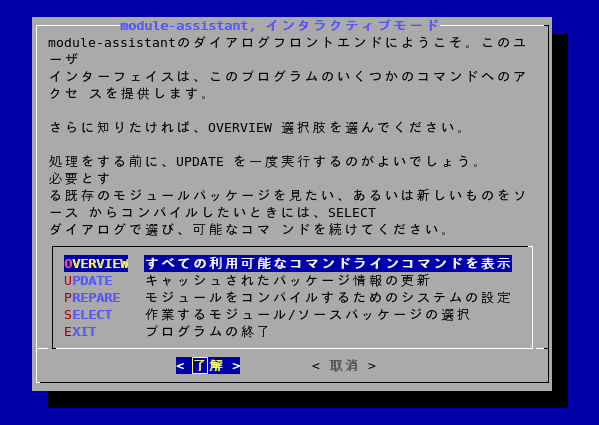
\includegraphics[width=1\hsize]{image200608/m-a.png}
\end{minipage}
\end{frame}

\begin{frame}
 \frametitle{使う側から}
 \begin{itemize}
  \item m-a prepare 
  \item m-a a-i パッケージ\\
	コンパイルしてパッケージを作成し、インストールするところまでやっ
	てくれる!
 \end{itemize}
\end{frame}

\begin{frame}
 \frametitle{作る側の視点 1/2}
 \begin{itemize}
  \item dh\_make 'k' を選択
  \item XXXX-source パッケージと XXXX-tool パッケージ(必須ではない)を
	作成
  \item XXXX-source 用に debian/ディレクトリを持つ
	\texttt{/usr/src/XXXX.tar.bz2} を作成するコードを仕込む。
 \end{itemize}
\end{frame}

\begin{frame}
 \frametitle{作る側の視点 2/2}
 \begin{itemize}
  \item control.modules.in など: \_KVERS\_ を置換
  \item rules: m-a 用のincludeをつっこんで、binary-modules でカーネルモ
	ジュールを
	\texttt{INSTALL\_MOD\_PATH=\$(CURDIR)/debian/\$(PKGNAME)} 以下にインストールするように。
 \end{itemize}
\begin{texttt}
-include \$(MA\_DIR)/include/generic.make\\
-include \$(MA\_DIR)/include/common-rules.make\\
\end{texttt}
\end{frame}

\begin{frame}
 \frametitle{罠}
 \begin{itemize}
  \item debian/rules が違う状況で実行されるのでそれなりにデバッグが複雑
	\\ パッケージをビルドしてインストールして \texttt{m-a a-i} して
	はじめてデバッグできる
  \item カーネルのモジュールの作成の仕組(kbuild)は数年に一回程度は大幅に
	変更されているので情報においつくのにそれなりに努力必要
  \item 自分が知らないデバイスが動かないというバグレポートがきても
	手のうちようが・・・
 \end{itemize}
\end{frame}

\begin{frame}
 \frametitle{まとめ}
 \begin{itemize}[<+->]
  \item ユーザ側から見て、module-assistant 便利
  \item module-assistant 用のパッケージの作成も簡単
  \item みんなカーネルモジュールをつくってパッケージにしよう!
 \end{itemize}
\end{frame}



\subsection{board@jpお仕事日記}
\begin{frame}
 \frametitle{board@jpお仕事日記
 \begin{itemize}
  \item ちょうどよい機会なのでどういうことをしてきたか
 \end{itemize}}
\end{frame}
\begin{frame}
 \frametitle{過去数年間}
 \begin{itemize}[<+->]
  \item \url{board@debian.or.jp} にくるSPAMをひたすら読む
  \item たまにくる雑誌などの問い合わせにこたえる
  \item 以下検閲削除
 \end{itemize}
\end{frame}

\begin{frame}
 \frametitle{今後}
 \begin{itemize}[<+->]
  \item 決めることはばっさばっさと決めていきます
  \item 御協力お願いします
 \end{itemize}
\end{frame}


\frame{\titlepage{}}

\section{グループワーク}

\begin{frame}
 \frametitle{今後のイベントの検討}
 \begin{itemize}
  \item Debian 勉強会の目的:
  \item イベントにより期待する効果:
  \item 必要な行動:
 \end{itemize}
\end{frame}

\begin{frame}
 \frametitle{今後のイベント}
 \begin{itemize}
  \item OSC 沖縄 12月1日?
  \item OSC-Fall 10月28日? 
  \item KOF 11月18日
  \item Debian 勉強会大阪開催 11月19日
  \item Debian Conference 2007 Edinburgh
  \item Debian 14周年 2007年8月16日
 \end{itemize}
\end{frame}

\section{wrap-up}
\begin{frame}
 \frametitle{今日のまとめ}
 \begin{itemize}
  \item 気づいたらすでに Debian 13周年です
  \item \texttt{module-assistant}活用してください。	
  \item コメントをメールで送ってください、あとでまとめます。
 \end{itemize}
\end{frame}

\end{document}
